\chapter{Website Designing}
The Smart Home Lab website consists of 5 web pages. Those are:
\begin{itemize*}
\item Home
\item The Lab
\item Components
\item Panels
\item Use Cases
\end{itemize*}

These web pages have been created and designed within the WordPress \cite{Williams.2015} by using a WordPress plugin called 'Page Builder By SiteOrigin'. This chapter will discuss on how these web pages has been created and designed, as well as the important steps and settings involved in it.

\section{Enabling Page Builder Plugin}
Firstly, the 'Page Builder by SiteOrigin' \cite{SiteOrigin.2016, SiteOrigin.2014} has to be downloaded and activated in the WordPress. This can be done through the 'Plugins' section in the admin side of the WordPress. After downloading and activating the plugin, the Page Builder plugin will automatically add a tab on the top right of the page editor (refer Figure~\ref{enabling-page-builder}), when a new page has been created. The usage of Page Builder can be enabled simply by clicking on this tab.

\begin{figure}[ht]
\centering
\caption{Enabling Page Builder Plugin}
\label{enabling-page-builder}
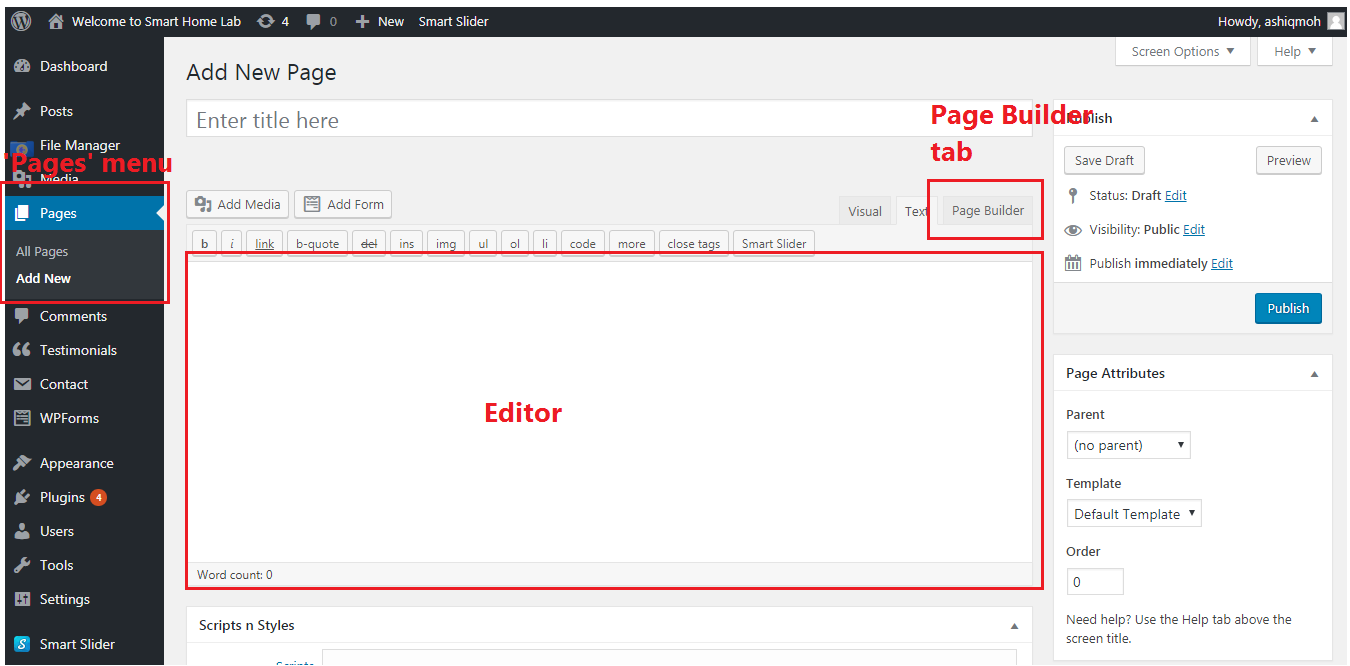
\includegraphics[height=5cm,keepaspectratio]{website-designing/enabling-page-builder.png}
\end{figure}

\section{Adding row, column and widget}
When Page Builder plugin has been enabled, the editor will display a series of buttons on the top of the editor. One of the important thing here is the 'Add Row' option. A row in the page builder signifies a horizontal section in a web page as shown in the Figure~\ref{row-section-explanation}. Each of this section is a row.

\begin{figure}[ht]
\centering
\caption{A row representing a horizontal column on the website}
\label{row-section-explanation}
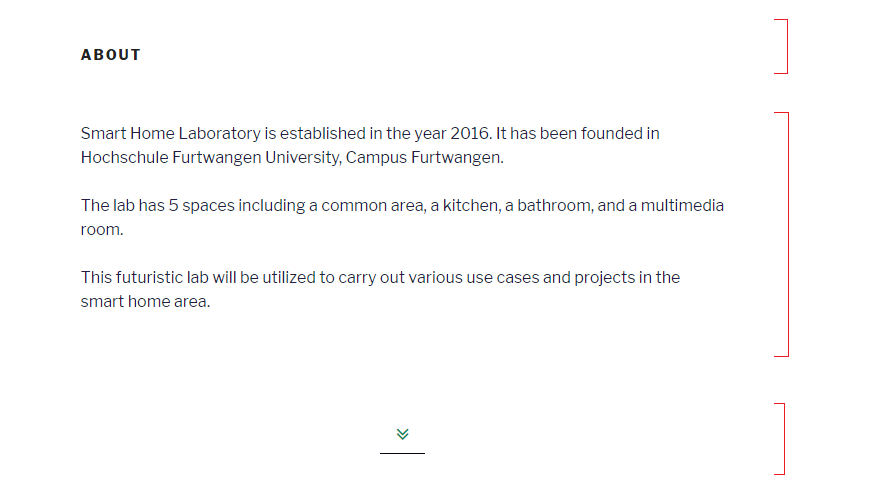
\includegraphics[height=5cm,keepaspectratio]{website-designing/row-section-explanation.png}
\end{figure}

When the 'Add Row' button (see~Figure \ref{adding-row}) is clicked, a new window (see Figure~\ref{adding-column}) will be opened asking to set the column. Here, the number of columns as well as the individual size of the column has to be given in.

\begin{figure}[ht]
\centering
	\begin{subfigure}{.49\linewidth}
	\centering
	\caption{Adding Row}
	\label{adding-row}
	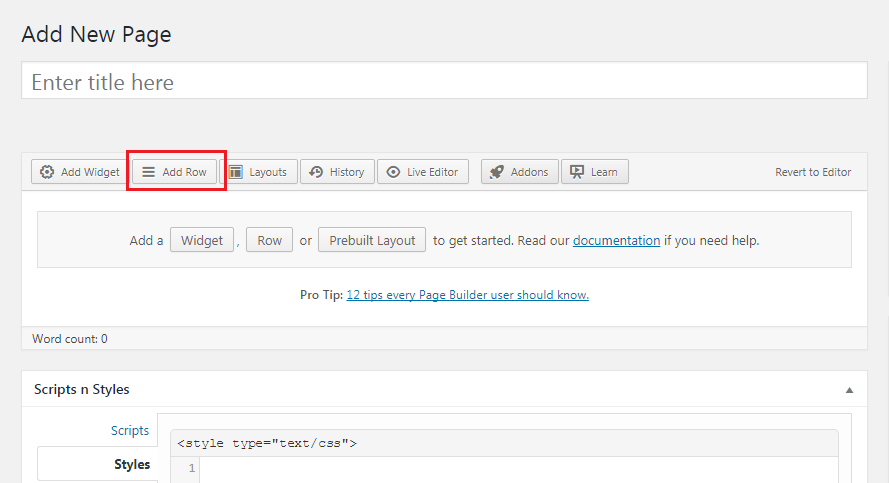
\includegraphics[width=\textwidth,keepaspectratio]{website-designing/adding-row.png}
	\end{subfigure}
	\begin{subfigure}{0.49\linewidth}
	\centering
	\caption{Adding Column}
	\label{adding-column}
	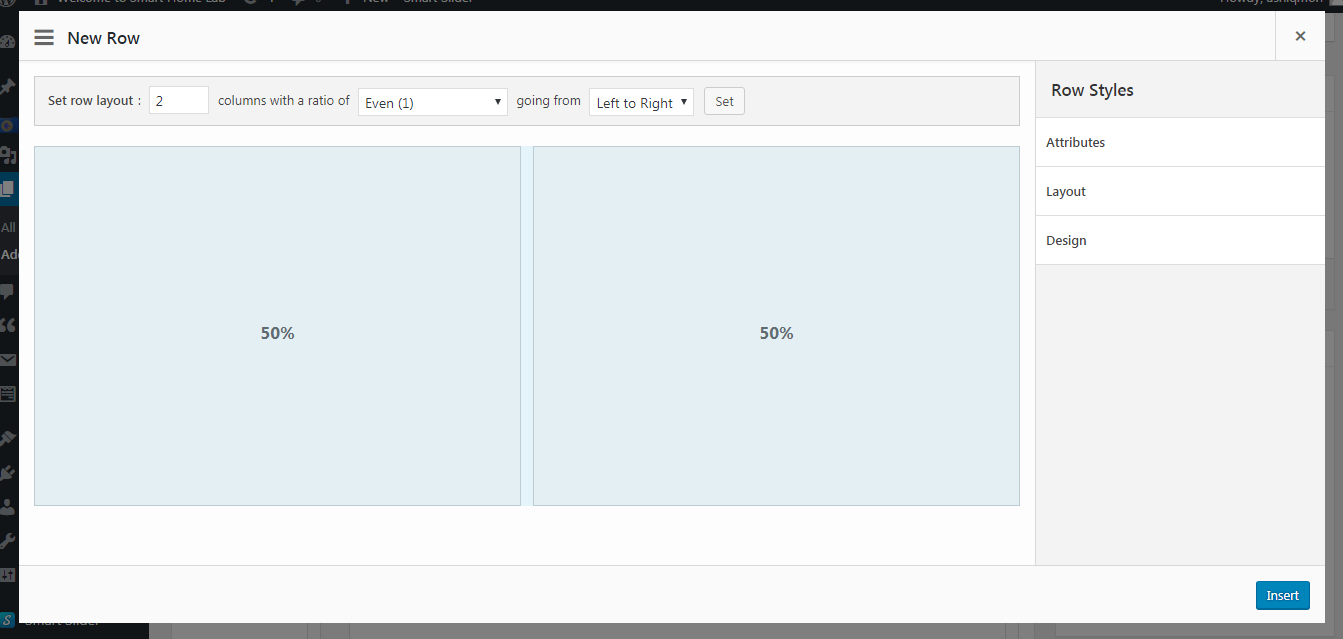
\includegraphics[width=\textwidth,,keepaspectratio]{website-designing/adding-column.png}
	\end{subfigure}
\end{figure}

After a row and a column (optionally multiple columns to a row) have been added, the editor will display a box within it. Within this box, widgets can be added by clicking the 'Add Widget' button next to the 'Add Row' button. When this button is clicked, a new window (see Figure~\ref{list-of-widgets} will pop up prompting which widget to be added into the created row i.e. column. The list of widgets consists of, for an example, 'SiteOrigin Editor', 'SiteOrigin Button', 'SiteOrigin Button' etc. To add normal text into the web page, one need to insert the 'SiteOrigin Editor' widget into the row. For a short note, multiple widgets can be inserted into a single row i.e. column.

\begin{figure}[ht]
\centering
\caption{Window showing a list of widgets to be inserted in to row i.e. column}
\label{list-of-widgets}
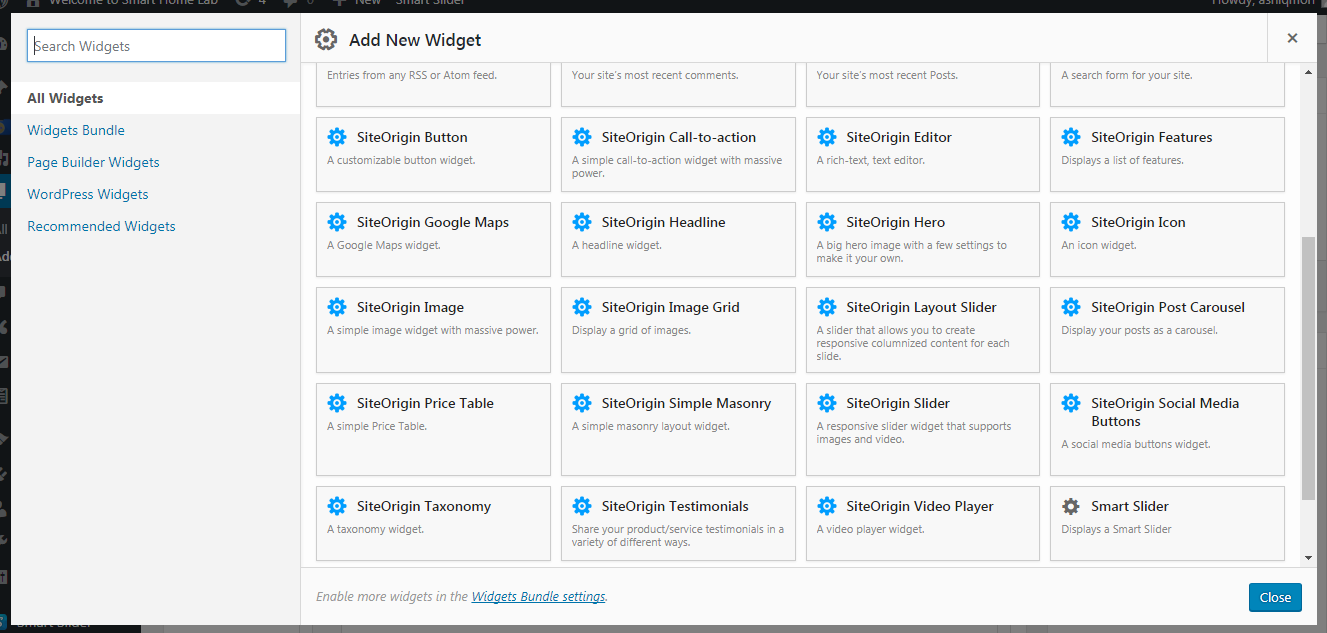
\includegraphics[height=5cm,keepaspectratio]{website-designing/list-of-widgets.png}
\end{figure}

Here is an example of screenshot of page builder row before and after adding a widget. In this example, the SiteOrigin Editor widget has been added.

\begin{figure}[ht]
\centering
	\begin{subfigure}{.49\linewidth}
	\centering
	\caption{Row before adding widget}
	\label{row-before-adding-widget}
	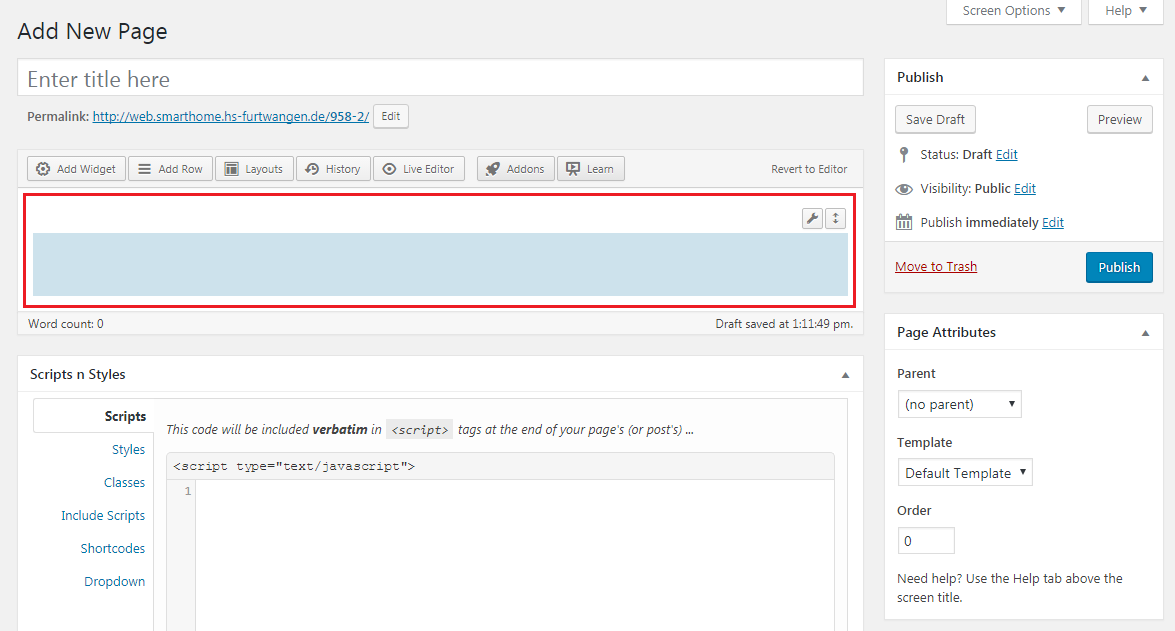
\includegraphics[width=\textwidth,keepaspectratio]{website-designing/row-before-adding-widget.png}
	\end{subfigure}
	\begin{subfigure}{0.49\linewidth}
	\centering
	\caption{Row after adding widget}
	\label{Row after adding widget}
	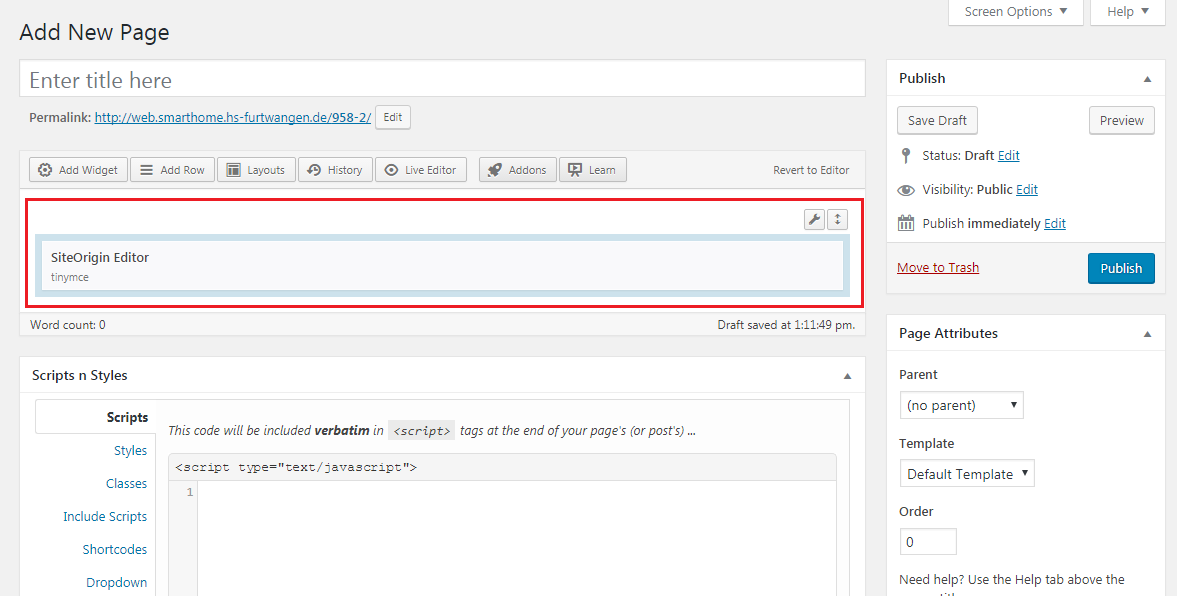
\includegraphics[width=\textwidth,,keepaspectratio]{website-designing/row-after-adding-widget.png}
	\end{subfigure}
\end{figure}

\section{Adding text, image and button}
Text can be added into the web page through the SiteOrigin Editor plugin. After the SiteOrigin Editor plugin has been inserted into the row/column, a menu list will appear when one hover the mouse over it. In the menu list, the 'edit' option has to be clicked to open the editor. In the editor, the text that has been intended to be added to web page can be typed. Text here can represent the header text and the normal paragraph text.

Next, in order to add an image, the SiteOrigin Image plugin can be used. After inserting the plugin, throught the edit option, a new window will be opened. Here, the URL of image as well as other settings such as image size, image alignment, image title etc. can be entered.

The button which are found on the web pages are added through the SiteOrigin Button plugin. Same as step above, after adding the plugin, one has to click on the 'edit' option on mouse over. Here, one has to define the destination URL which will be opened when the button is clicked. Optionally, the text or icon that should appear on the button can be added. There are also other options for alignment layout designing of the button.

\section{Adding Scroll Effect}
As can be noticed, clicking on the button scroll the content to a specific part of the web page. To enable the scroll effect, a few steps have to be taken.

First, a plugin called 'Page Scroll to Id' has to be added and activated in the WordPress. After adding and activating, buttons that have been added has to be given the class name 'ps2id'. The class name of a button can be given by the 'edit' option mentioned in the previous section. In the edit section, under the 'Other attributes and SEO', the class name can be given in the 'Button Classes' field as can be seen in the Figure~\ref{button-class-name}.

\begin{figure}[ht]
\centering
\caption{Button Classes field where 'ps2id' has to be entered}
\label{button-class-name}
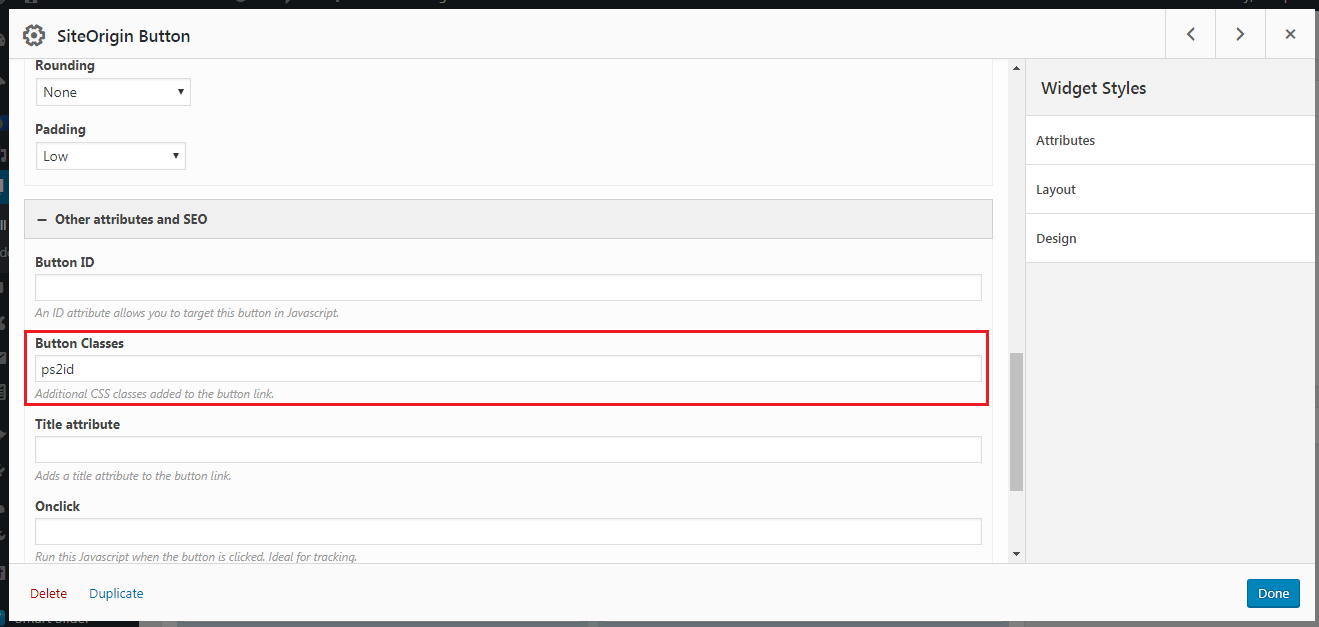
\includegraphics[height=5cm,keepaspectratio]{website-designing/button-class-name.png}
\end{figure}

Lastly, the destination URL has to be set. The destination \ac{url} has to be entered in two places. First in button edit section, under the 'Destination URL' field as can be seen in the Figure~\ref{destination-url-button}.  Secondly, the same destination URL has to be given to 'Row ID' field of the target element. The step to provide the target element an id is shown in the Figure~\ref{target-element-id}. By assigning the button and the target element the id, the button will scroll the web page to target element.

\begin{figure}[ht]
\centering
\caption{Adding the destination URL for a button}
\label{destination-url-button}
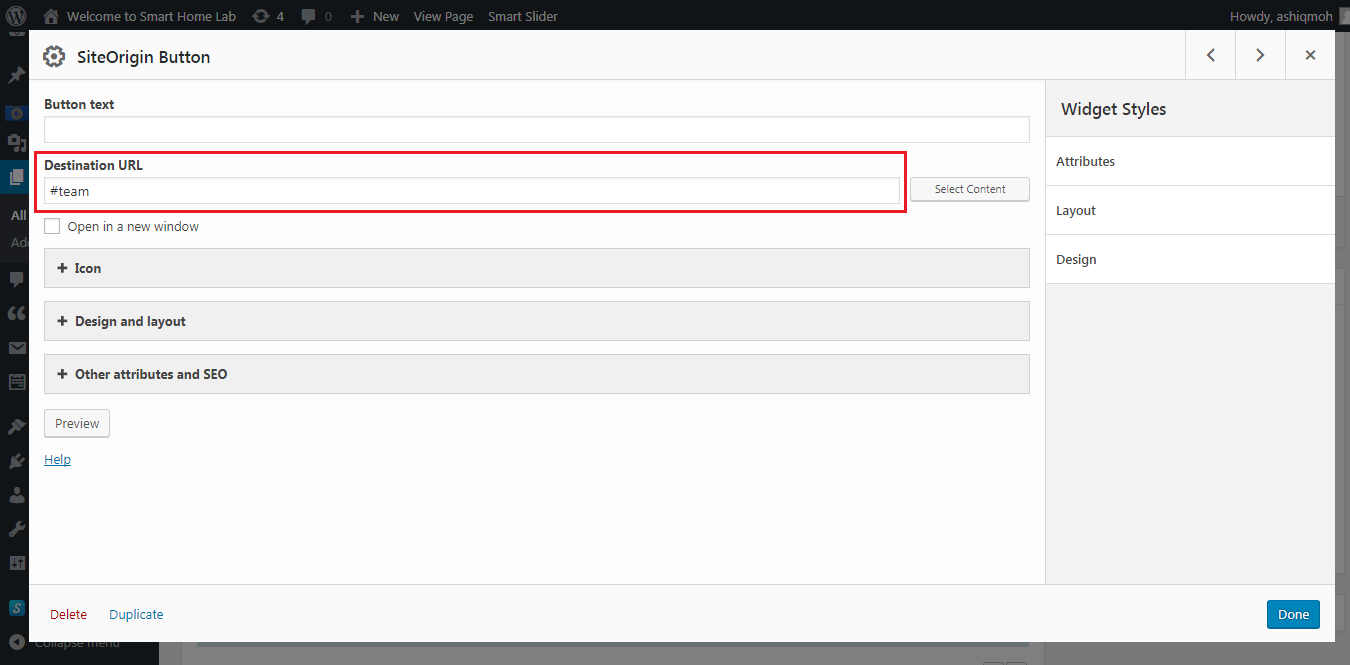
\includegraphics[height=5cm,keepaspectratio]{website-designing/destination-url-button.png}
\end{figure}

\begin{figure}[ht]
\caption{Adding Row Id to the Target Element}
\label{target-element-id}
\centering
	\begin{subfigure}{.49\linewidth}
	\centering
	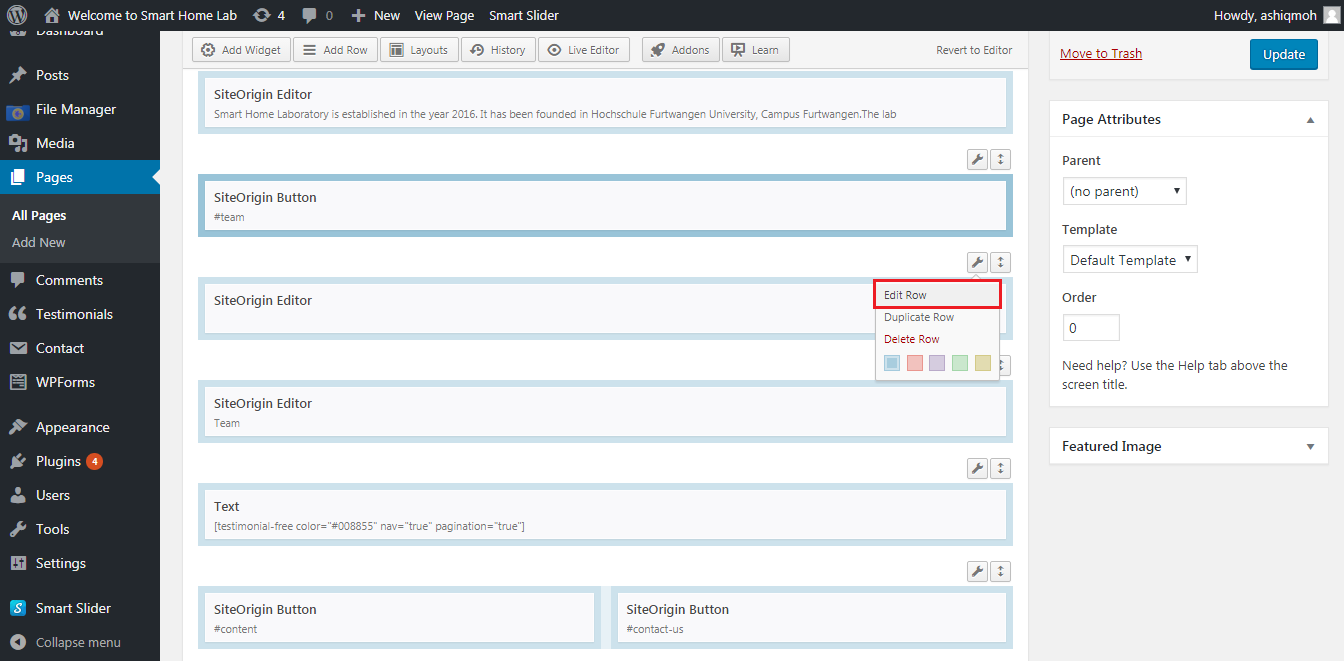
\includegraphics[width=\textwidth,keepaspectratio]{website-designing/destination-url-1.png}
	\end{subfigure}
	\begin{subfigure}{0.49\linewidth}
	\centering
	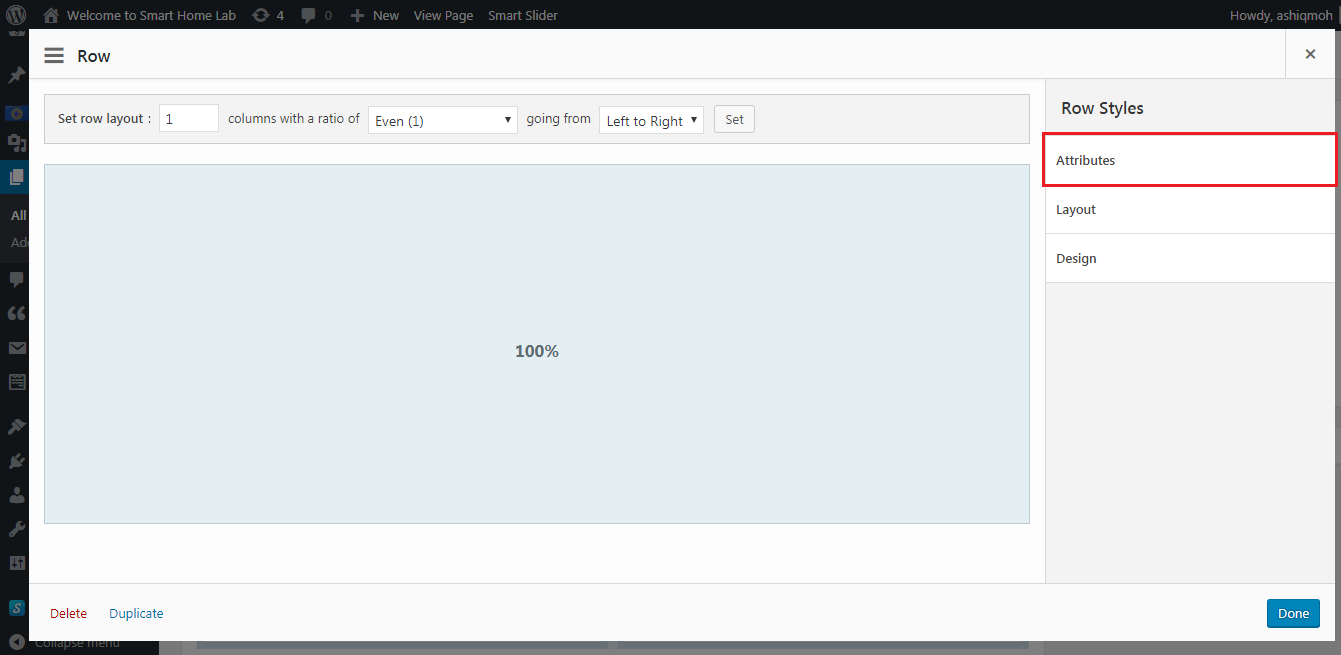
\includegraphics[width=\textwidth,,keepaspectratio]{website-designing/destination-url-2.png}
	\end{subfigure}
	\begin{subfigure}{0.49\linewidth}
	\centering
	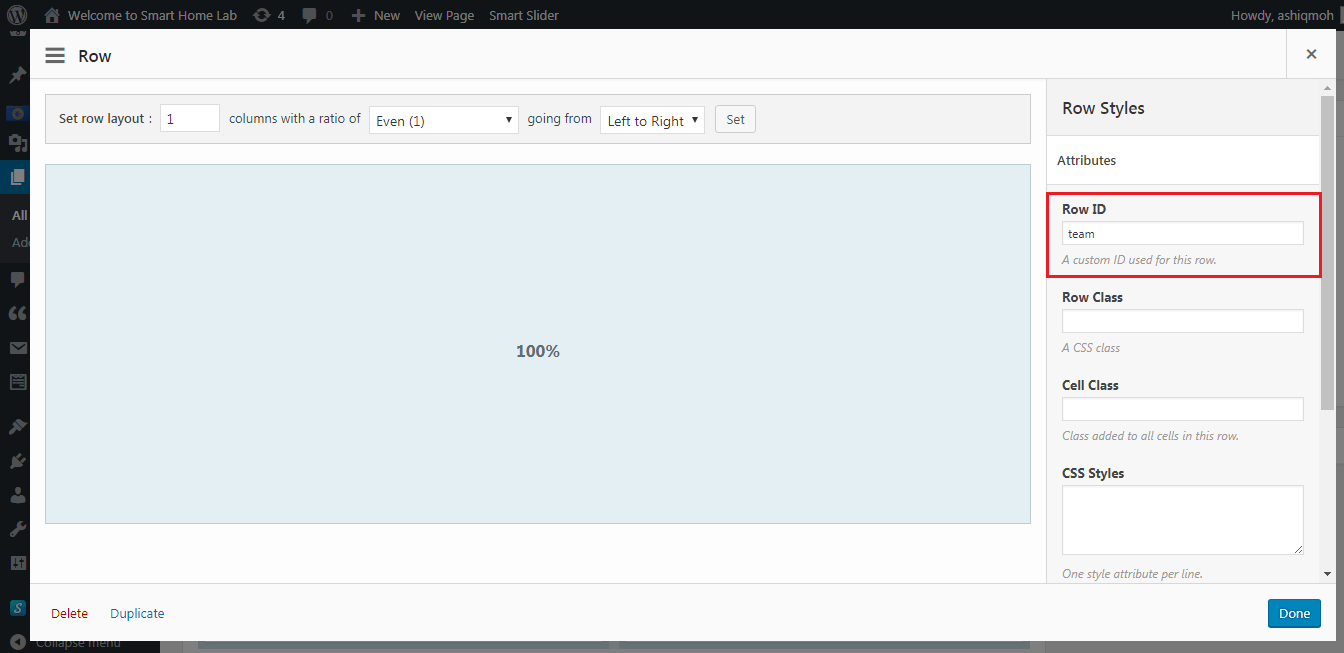
\includegraphics[width=\textwidth,,keepaspectratio]{website-designing/destination-url-3.png}
	\end{subfigure}
\end{figure}

\section{Adding ScrollReveal Effect}
ScrollReveal effect is an effect that can be added to the content of a web page, where the content will get an animation or effect that it is being revealed to the users as they scroll down or up through the page. This effect can be added to any website through importing a JavaScript library, ScrollReveal written by Julian Lloyd\footnote{https://scrollrevealjs.org/}.

This section will explain how to add this effect to a WordPress page. First, a plugin called 'Scripts n Styles'\footnote{https://wordpress.org/plugins/scripts-n-styles/} has to be added and activated in the WordPress. After activating the plugin, the 'Page' section in the WordPress will receive a new screen option under the editor, where JavaScript and CSS code can be added as shown in the Figure~\ref{scripts-n-styles}.

\begin{figure}[ht]
\centering
\caption{Scripts n Styles screen option}
\label{scripts-n-styles}
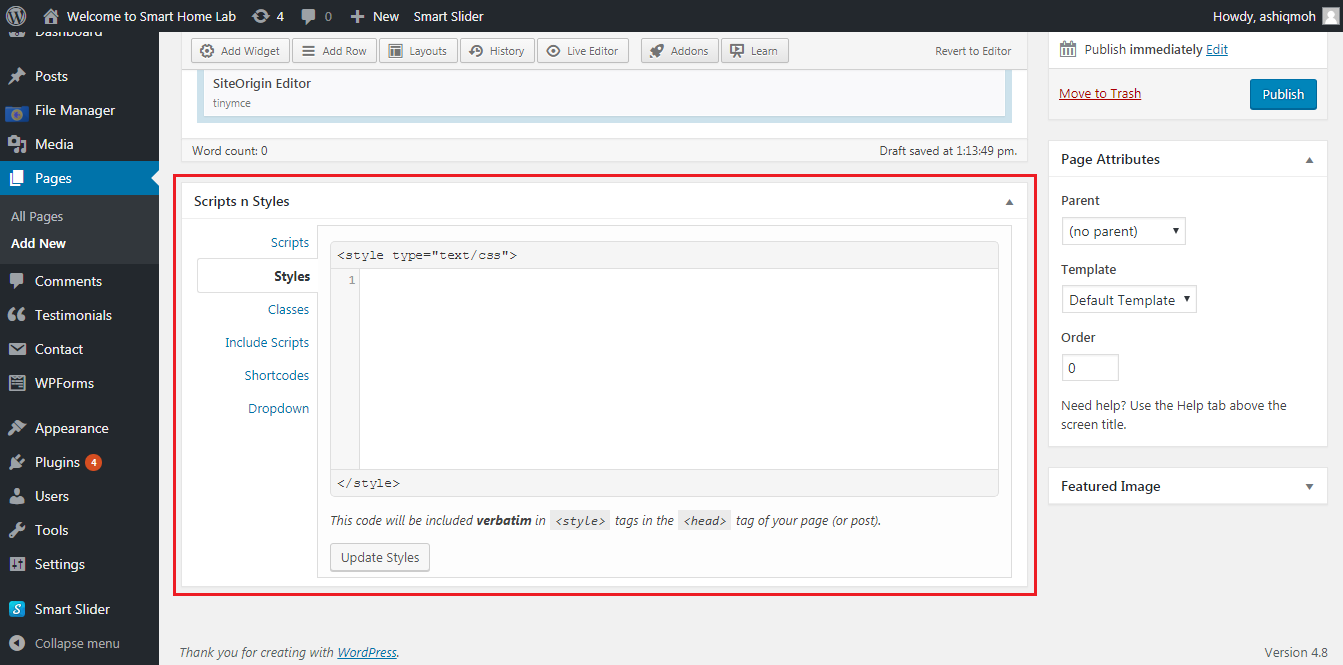
\includegraphics[height=5cm,keepaspectratio]{website-designing/scripts-n-styles.png}
\end{figure}

Here, the script tab has to be clicked so that our own JavaScript can be added to the current page. There, the plugin offers two option of adding JavaScript codes to current web page. Either at the header part of web page at the top, or at body part of the web page at the bottom. Here, the codes required to enable ScrollReveal effect will be added at the body of the web page at the bottom.

\begin{figure}[ht]
\centering
\caption{Adding JavaScript to bottom of page}
\label{javascript-bottom-column}
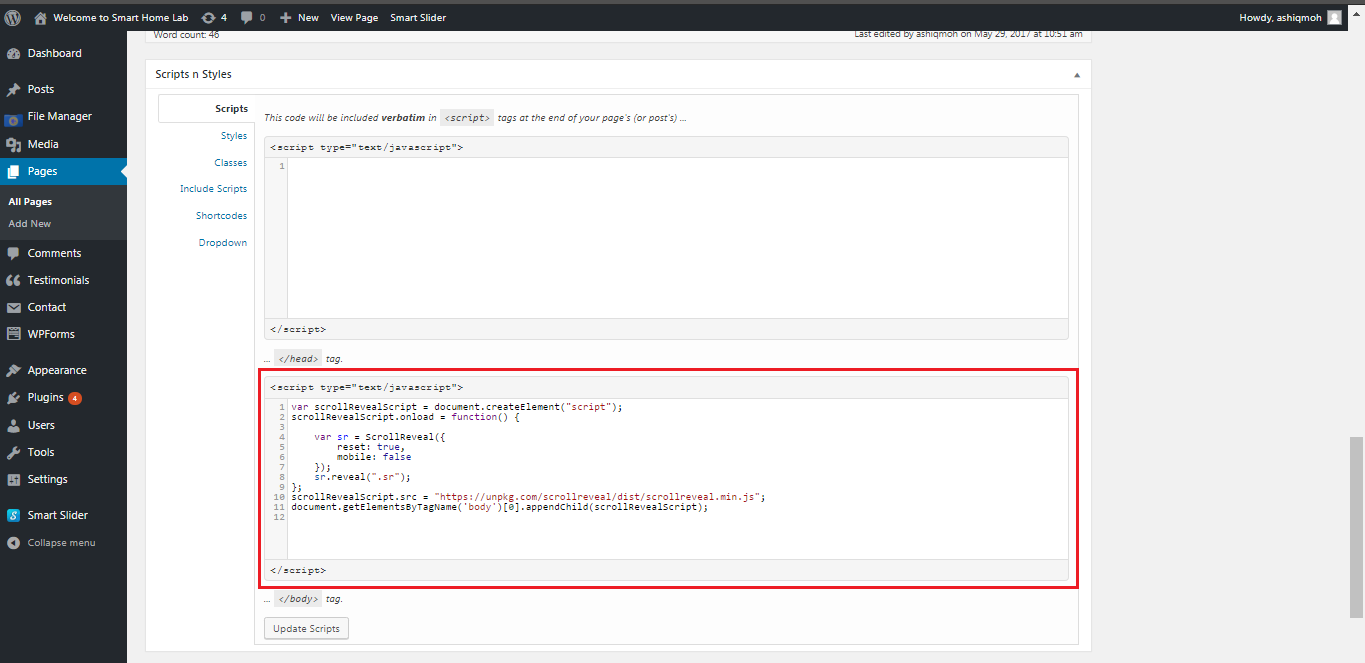
\includegraphics[height=5cm,keepaspectratio]{website-designing/javascript-bottom-column.png}
\end{figure}

The JavaScript codes that has been added will do two tasks. First, it will import the ScrollReveal library script from \ac{cdn} and insert it to current web page.

Secondly, the JavaScript code will be written to declare and initiate the ScrollReveal object, so that any HTML element assigned will receive the effect. Here, the elements with class name 'sr' has been assigned to get the ScrollReveal effect. The class name in JavaScript is identified with the punctuation mark '.' in the beginning. This has been done using the method \texttt{.reveal('.sr');}.

\begin{lstlisting}
var scrollRevealScript = document.createElement("script");
scrollRevealScript.onload = function() {

    // declare and initiate ScrollReveal object
    var sr = ScrollReveal({
        reset: true,
        mobile: false
    });
    // assign element that should receive the effect
    sr.reveal(".sr");
};
// import ScrollReveal library from CDN
scrollRevealScript.src = "https://unpkg.com/scrollreveal/dist/scrollreveal.min.js";
// insert the imported library into the web page
document.getElementsByTagName('body')[0].appendChild(scrollRevealScript);
\end{lstlisting}

The final step that has to be taken in order to enable the effect is to add the class name, in this case 'sr' to the HTML elements. This class name will be entered in the 'Row Class' field as shown in the Figure~\ref{class-name-sr}.

\begin{figure}[ht]
\caption{Adding Class Name to HTML Element}
\label{class-name-sr}
\centering
	\begin{subfigure}{.49\linewidth}
	\centering
	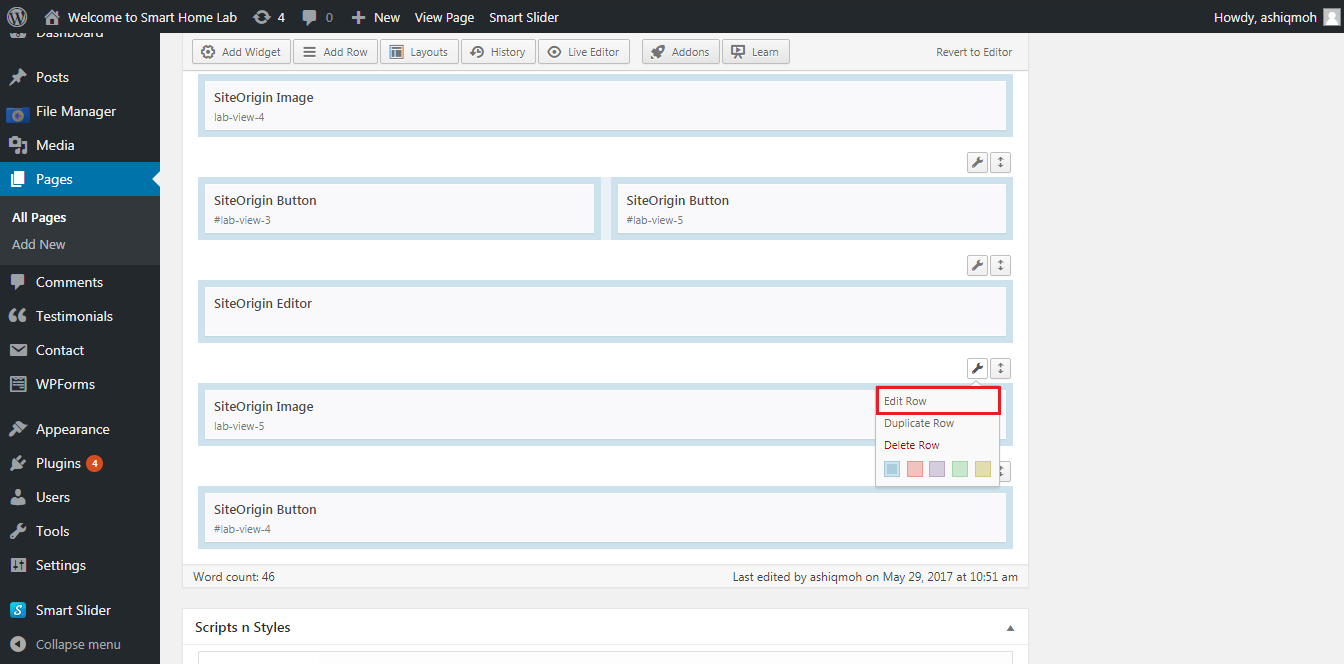
\includegraphics[width=\textwidth,keepaspectratio]{website-designing/class-name-sr-1.png}
	\end{subfigure}
	\begin{subfigure}{0.49\linewidth}
	\centering
	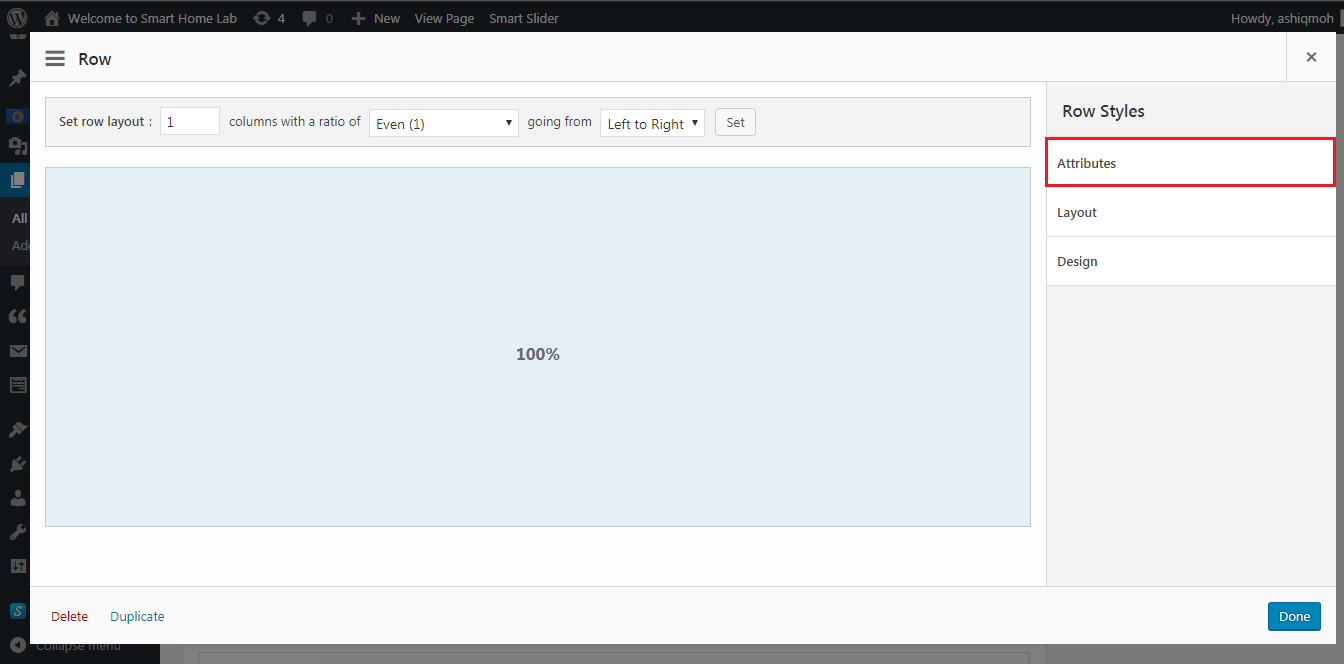
\includegraphics[width=\textwidth,,keepaspectratio]{website-designing/class-name-sr-2.png}
	\end{subfigure}
	\begin{subfigure}{0.49\linewidth}
	\centering
	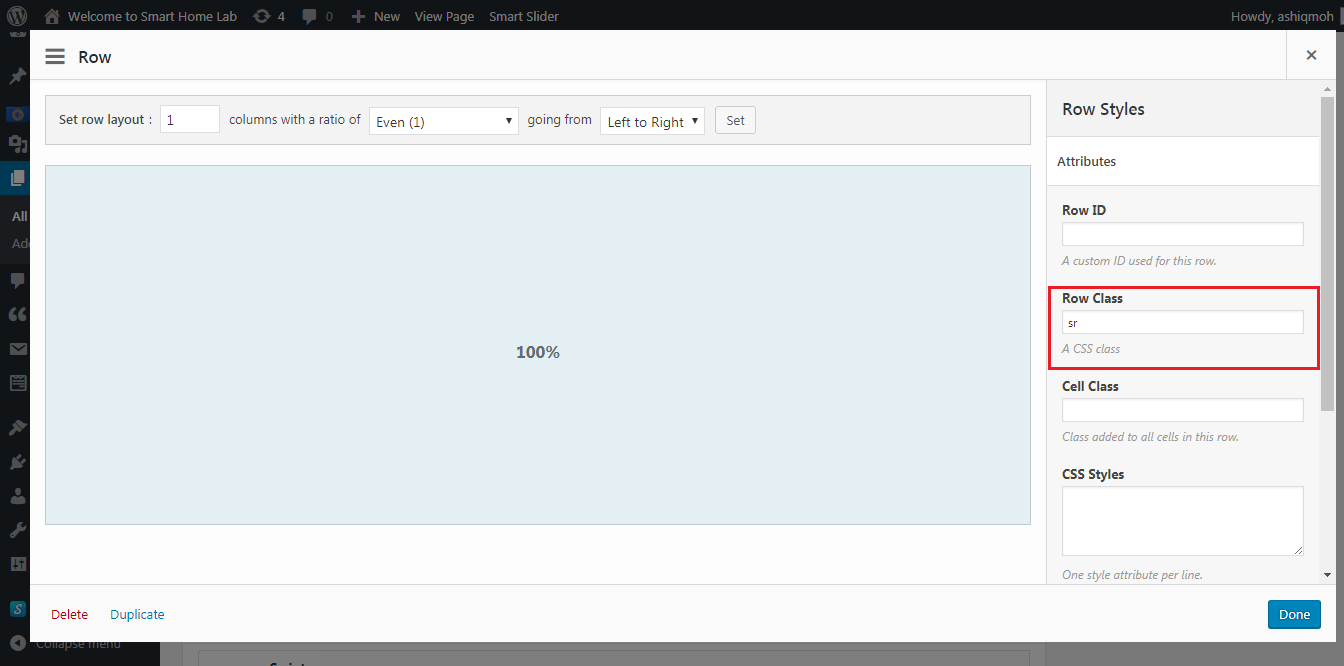
\includegraphics[width=\textwidth,,keepaspectratio]{website-designing/class-name-sr-3.png}
	\end{subfigure}
\end{figure}

